\documentclass[12pt,a4paper]{article}
\usepackage[utf8]{inputenc}
\usepackage{amsmath}
\usepackage{amsfonts}
\usepackage{amssymb}
\usepackage{graphicx}
\usepackage{float}
\usepackage{dsfont}
\usepackage{xcolor}
\usepackage[left=3.00cm, top=2.00cm, bottom=2.00cm]{geometry}
\author{Victor Todd-Moir\\Københavns Universitet}
\date{dd-mm-åå}
\title{Titel}
\begin{document}
	\maketitle
\section*{Data analysis}
We would like to predict the prices of games using a regression model. We will in the following scale our features to zero mean and unit variance. Afterwards we will perform a principal component analysis (PCA) in order to reduce the amount of features taken into consideration and thus we will account for a degree of overfitting. We will like to keep 90$\text{\%}$ of the variance in our training data. This is done by looking at the explained variance ratio of each feature and keeping the features with most explained variance ratio until we reach our threshold of 0.90. Afterwards we will fit an elastic net-model to our training data using 10-fold cross validation and perform a grid search to tune our hyperparameters of the elastic net-model. The hyperparameters are $\lambda$ and $\alpha$. $\lambda$ is the penalty term that penalizes the amount of features in our model and $\alpha$ determines the convex combination of LASSO penalization and Ridge penalization.\\
First we take a look at our dataset. Our target is 'price'. We drop the features 'name', 'release\_date', 'developer' and 'id' to create our feature matrix. Then we split our data into training and test date with a 80-20 ratio. Then we scale our training data. This is done to make sure that features of different magnitude are taken equally account for when fitting our model. As we have $453$ features to begin with one can easily imagine that a lot of our features would be made redundant without scaling, as we have many binary features and several numeric features of different magnitude in our data. The scaling is done with the sklearn.preprocessing.StandardScaler class. Next we perform a principal component analysis on our training data. We start by including $453$ components. This way we can for each component see how much of the explained variance each component contributes to the full variance of the training data. Below we see a figure of the cummulative sum of explained variance ratio as a function of the number of eigenvectors to include\\
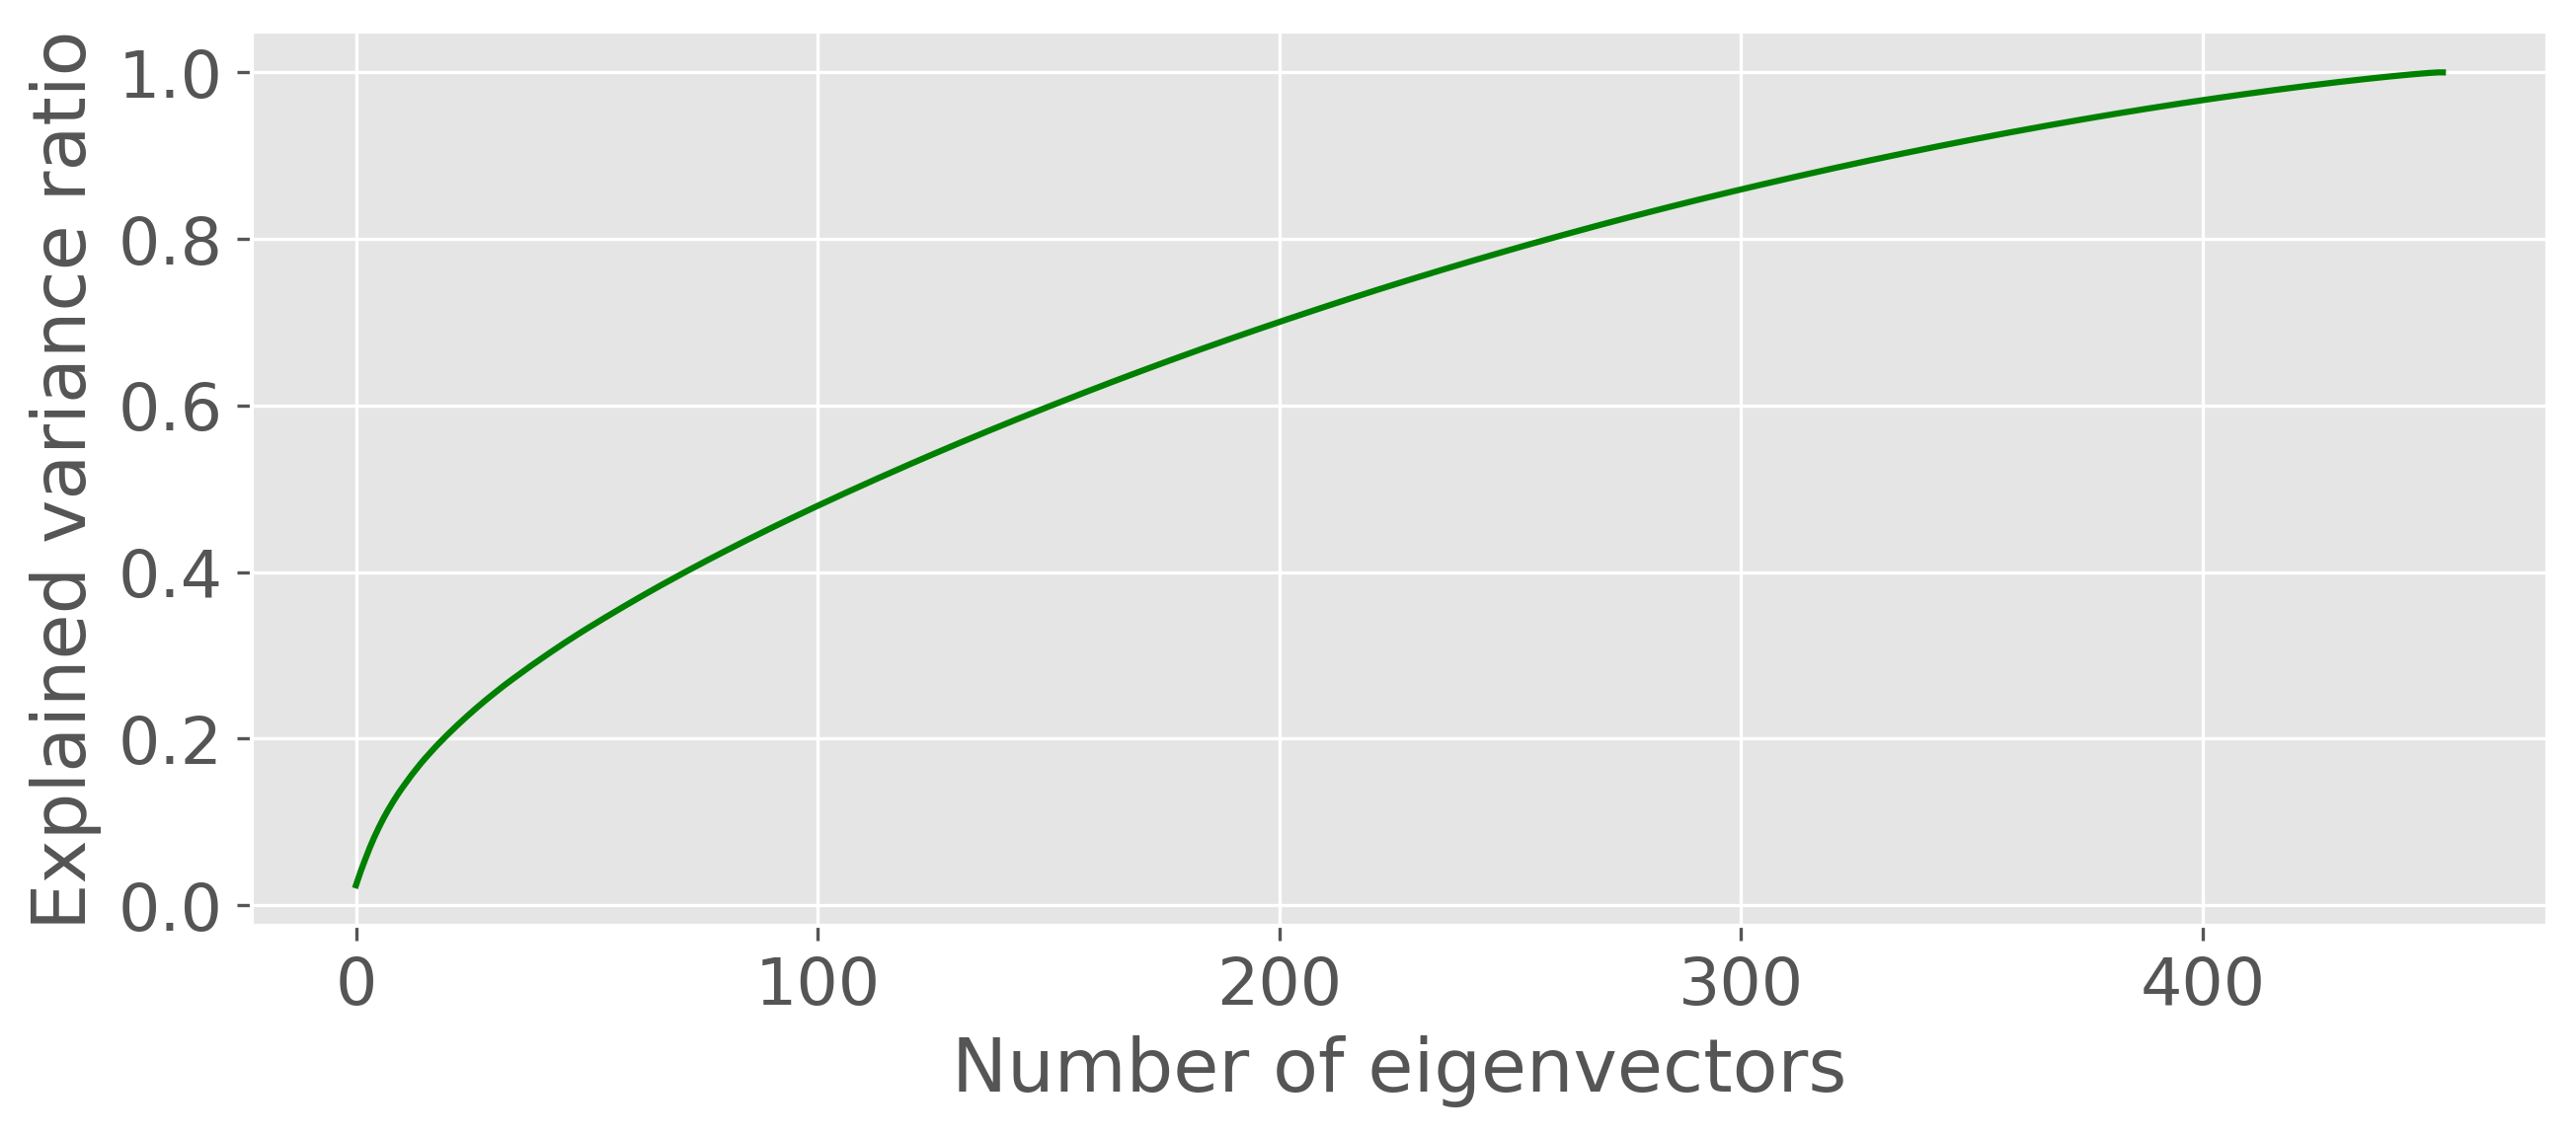
\includegraphics[scale = 0.5]{cumsumEigen.png}
\\
To keep our threshold of 0.90\% of the variance, we find that we must have 334 components in our final model. We see that we lower our dimension of features by approximately one fourth. PCA is done to avoid too much overfitting while still maximizing variance in the dataset. The PCA is done with the sklearn.decomposition.PCA class.\\
We will now look at LASSO regression and Ridge regression seperately. Regression is a supervised learning method that seeks to find weights for all features such as to minimize the predicted target of an observation and the true value. A prediction has the following form
$$\hat{y} = \boldsymbol{w}^\intercal \boldsymbol{x}$$
(INCLUDE REFERENCE TO PML, CHAP 10, PDF PAGE 451)Both LASSO and Ridge penalize the amount of features we keep in a final model. LASSO regression seeks to minimize the following function:
$$J(w)_{LASSO} = \sum_{i = 1}^{N}(y_i - \hat{y}_i)^2 + \lambda \sum_{j=1}^{m}|w_m|$$
Note that $N$ is the number of observations, $m$ is the number of features and $\lambda >0$ is a hyperparamter. The first sum is referred to as the sum of squared errors (SSE). The second is our penalty term. LASSO penalizes the absolute value of our weights. To tune our hyperparameter $\lambda$ we perform 10-fold cross validation on our training data with different values of $\lambda$, where
$$\lambda \in [0.0001, 10000]$$ 
For each value of $\lambda$ we compute the mean squared error (MSE) on the validation set and averaging over all 10 folds. Performance for each $\lambda$ can be seen here\\
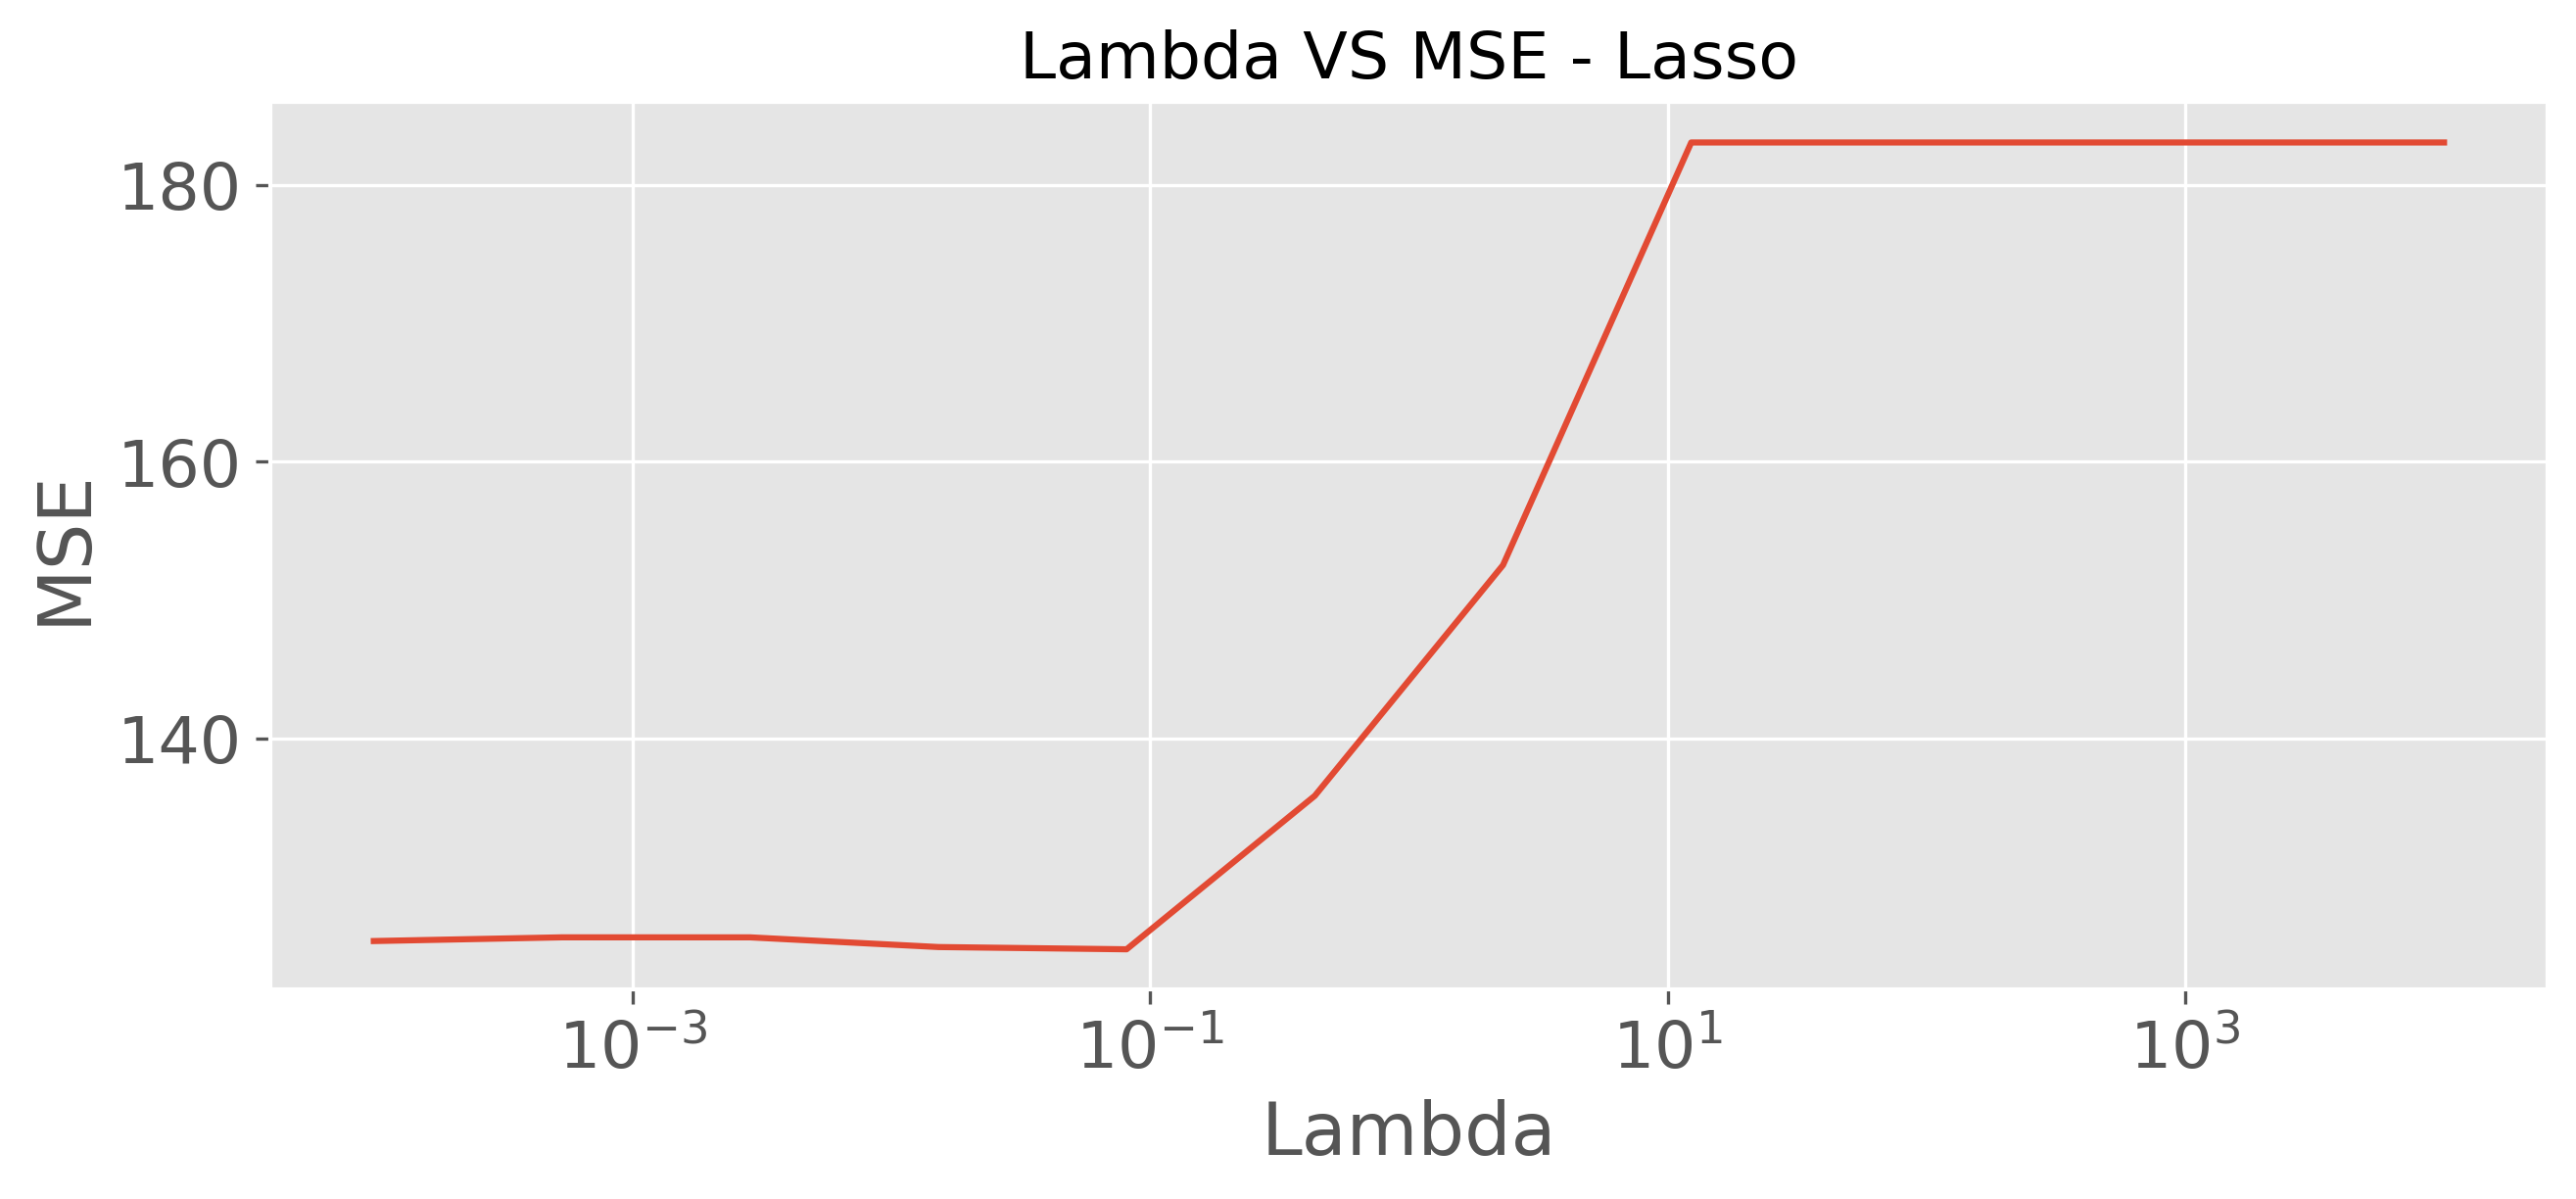
\includegraphics[scale = 0.7]{Lasso_MSE.png}
\\
Note the optimal $\lambda$, $\lambda^*_{LASSO} = 0.081113$, which yields an MSE of $124.8$. \\

Ridge regression seeks to minimize another function quite similar to the LASSO, namely:
$$J(w)_{Ridge} = \sum_{i = 1}^{N}(y_i - \hat{y}_i)^2 + \lambda \sum_{j=1}^{m}w_m^2$$
The SSE is the same but Ridge penalizes the squared value of our weights. We do the same procedure as previously described to tune our hyperparameter, $\lambda$. We search within the same space as before and find the optimal $\lambda$, $\lambda^*_{Ridge} = 1873.8$, which yields an MSE of $124.3$. Performance for each $\lambda$ can be seen here\\
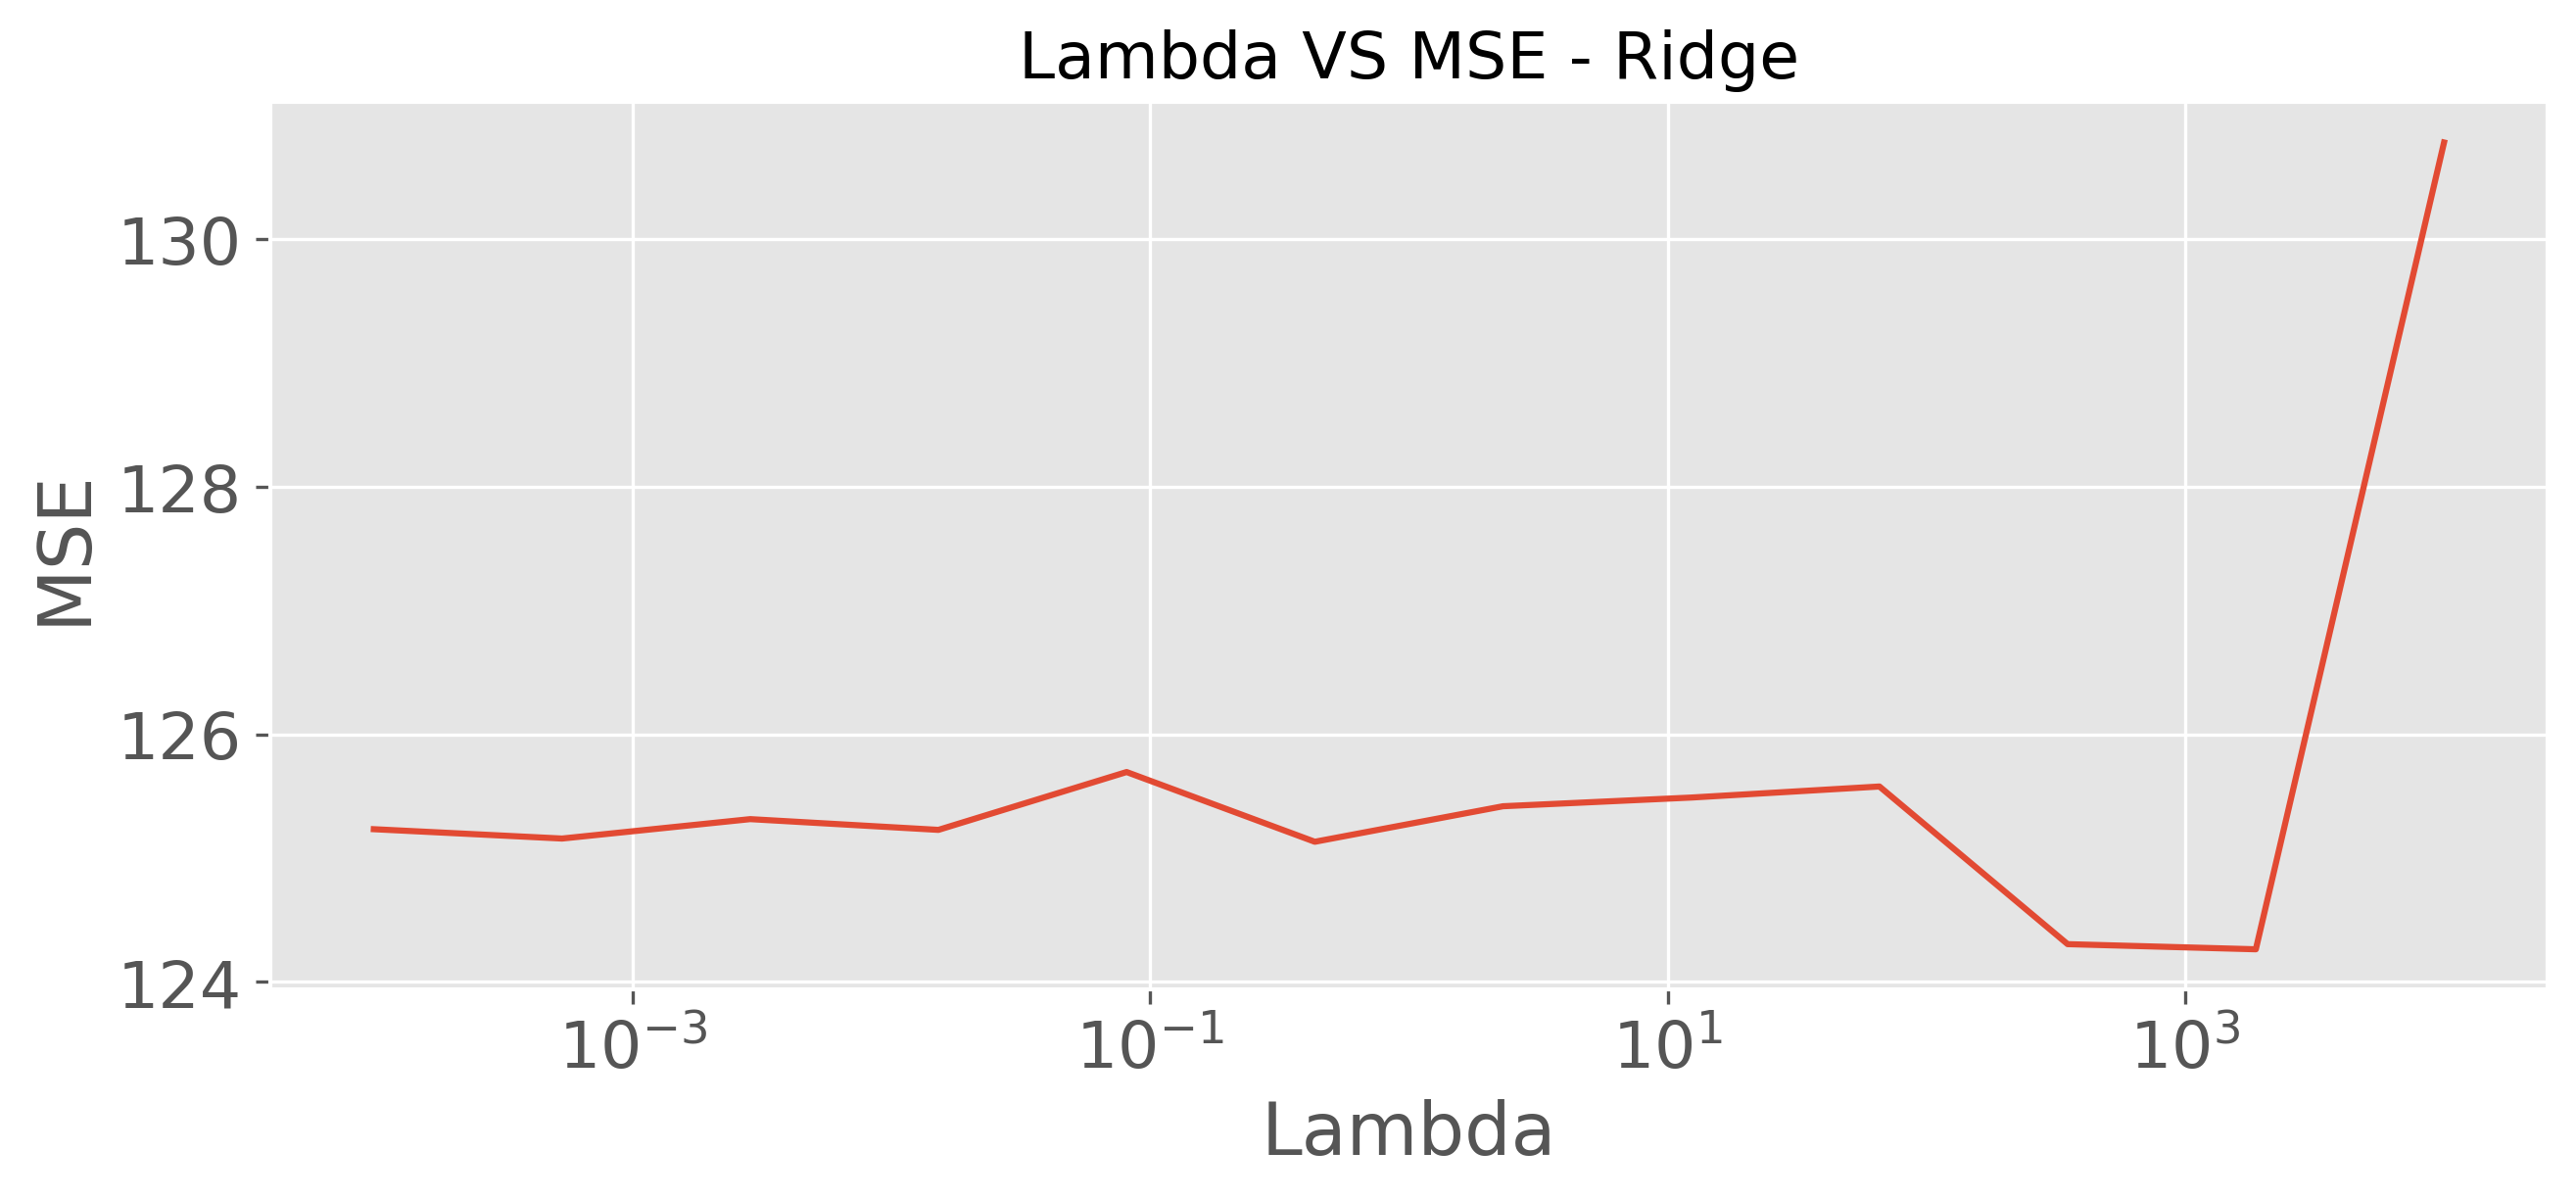
\includegraphics[scale = 0.7]{Ridge_MSE.png}
\\
All in all we see that the two types of regressions yield approximately the same MSE but two very different orders of magnitude for the optimal hyperparameter. 


\end{document}
